\section{Multilayer Perceptron}

\subsection{Methods}
This section covers how we went about implementing the MLP back-progagation gradient descent algorithm and which parameters we chose to make to make it perform well on the validation set.

\subsubsection{Treatment of Data}
First of all, before passing it on to the algorithm and training, we had to process the raw data of labelled digits.
\paragraph{Splitting}
The data was already separated into training and test data containing the pattern vectors for the digits and the corresponding classification labels. All what was left to do according to the instructions received was to split the training data into a random $\frac{2}{3}$ training and a $\frac{1}{3}$ validation set. This was easily achieved by randomly permuting the indices of the training data patterns and then dividing both the set of patterns and the set of labels at the $\frac{2}{3}$ mark according to the permutation.
\paragraph{Preprocessing}
Before starting off with training the MLP it had to be ensured that both training and validation set were properly normalized. As given in the project description, we computed the min. and max. values for every component of the untouched training patterns beforehand and then applied the normalization to the training and the test data. This preprocessing was actually done before splitting the data in order to save the operation on the validation set.

\subsubsection{MLP setup}
The structure of the MLP we were advised to use through the project instructions is depicted in Fig. \ref{fig:mlp}. The differences to the two-layer MLP discussed in the lecture lie in the following properties: Firstly, the first hidden layer has double the outputs than a "normal" MLP perceptron. Secondly, the gating function $g(a_{2k-1}, a_{2k})=a_{2k-1}\sigma(a_2k)$ takes pairs of values from the hidden layer accordingly. Lastly, the activation value $a^{(2)}$ is not passed through another gating function.
\begin{figure}[!h]
	\centering
	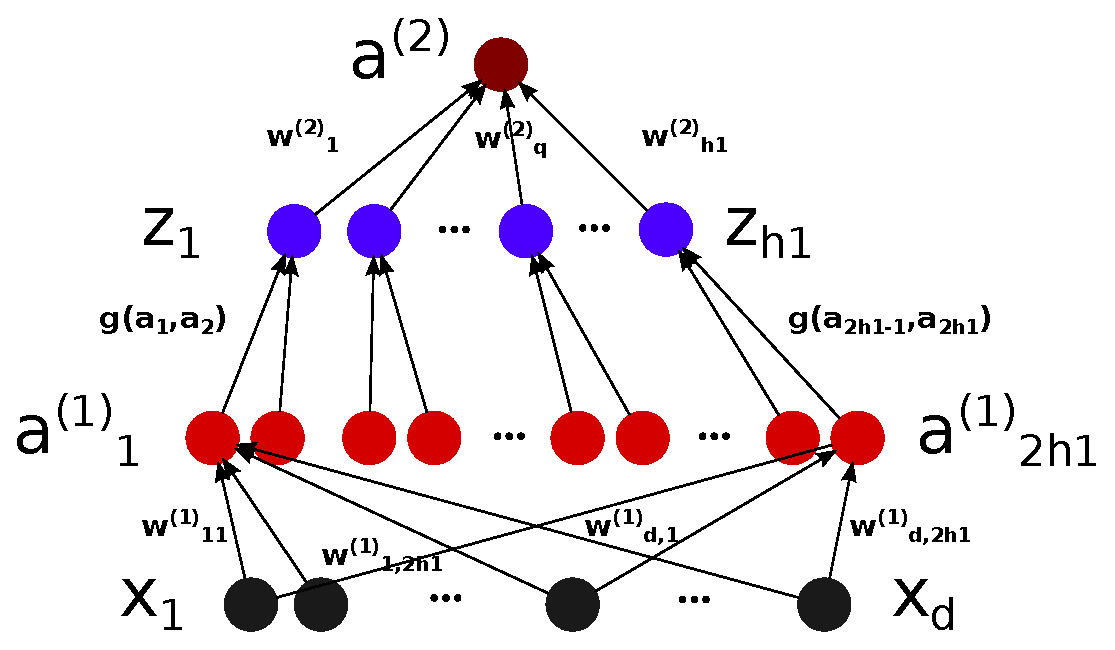
\includegraphics[width=.6\textwidth]{mlp/mlp.eps}
	\label{fig:mlp}
	\caption{Schema of the MLP described in the project instructions}
\end{figure}
Once we had the code for this setup running in python, we left the number of hidden layers and the gating function untouched and proceeded with the optimization of the remaining paramters, the number of hidden inputs $h_1$, the learning rate $\eta$ and the momentum term $\mu$. The discussion of the effects of the adjustment of these parameters is discussed with early stopping meaning that the optimization stops as soon as the validation error starts increasing.
%\paragraph{Early stopping}
%Evaluate empirical error $\hat{R}(\hat{f};\mathcal{D}_V)$ for validation set $\mathcal{D}_V$ along-side the training-error $\hat{R}(\hat{f};\mathcal{D}_T)$while training the MLP on $\mathcal{D}_T$. Stop at the training at the epoch where the validation error stops decreasing and starts increasing. 
%Show comparative plots illustrating the effects of learning rate, number of hidden units, momentum, etc. on\\
\paragraph{Effects of parameters on convergence speed and errors}
\begin{itemize}
	\item In fig. \ref{fig:effects_learning_rate} we show the effects of the learning rate $\eta$ and the momentum term $\mu$ on the convergence speed and the accuracy of the MLP classifier. 
		\begin{figure}[!ht]
		\centering
		\begin{subfigure}[b]{.45\textwidth}
		\centering
		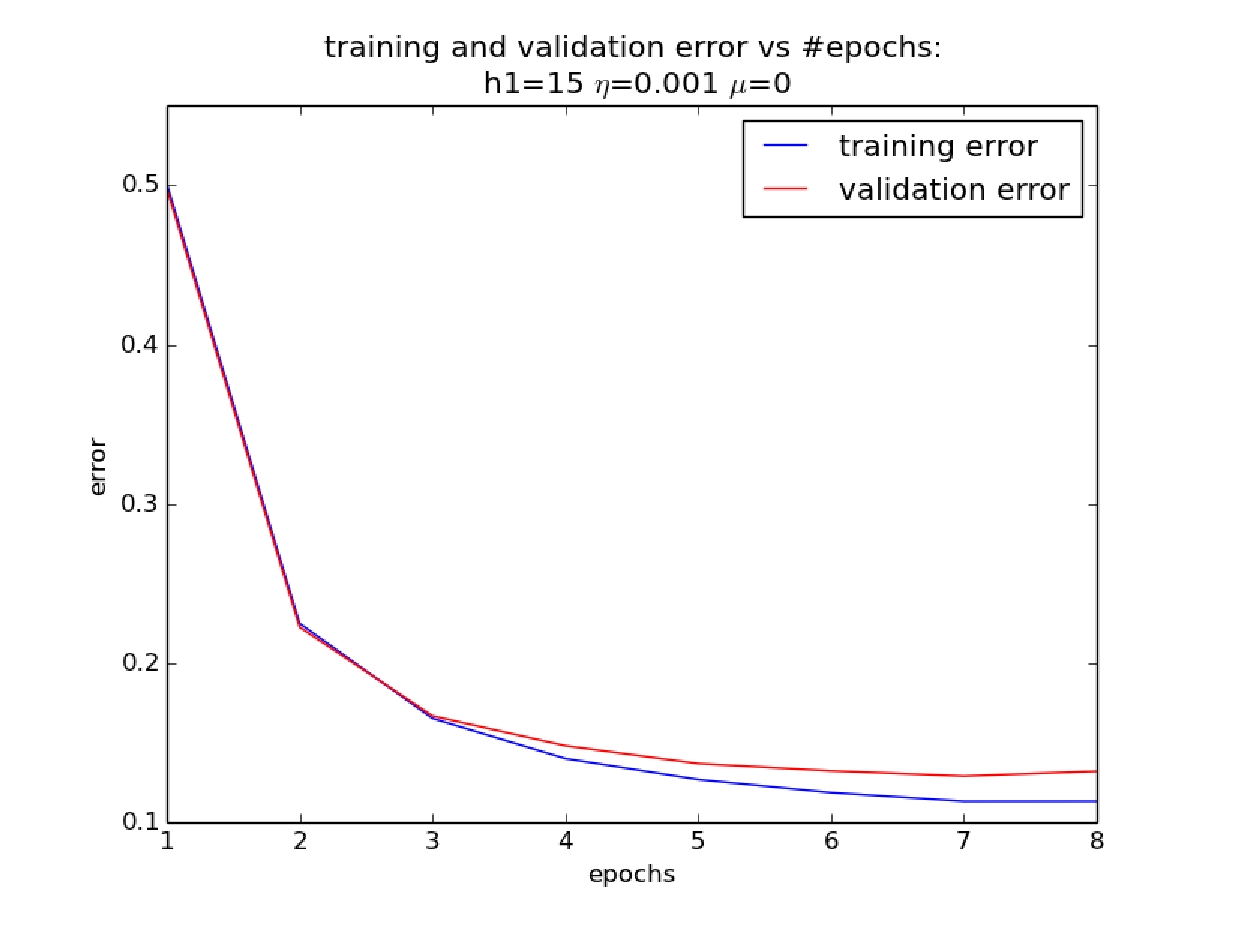
\includegraphics[width=\textwidth]{mlp/plots/effect_eta_small.eps}
		\caption{Errors with small $\eta_0=0.001$}
		\label{fig:small_eta}
		\end{subfigure}
		\quad
		\begin{subfigure}[b]{.45\textwidth}
		\centering
		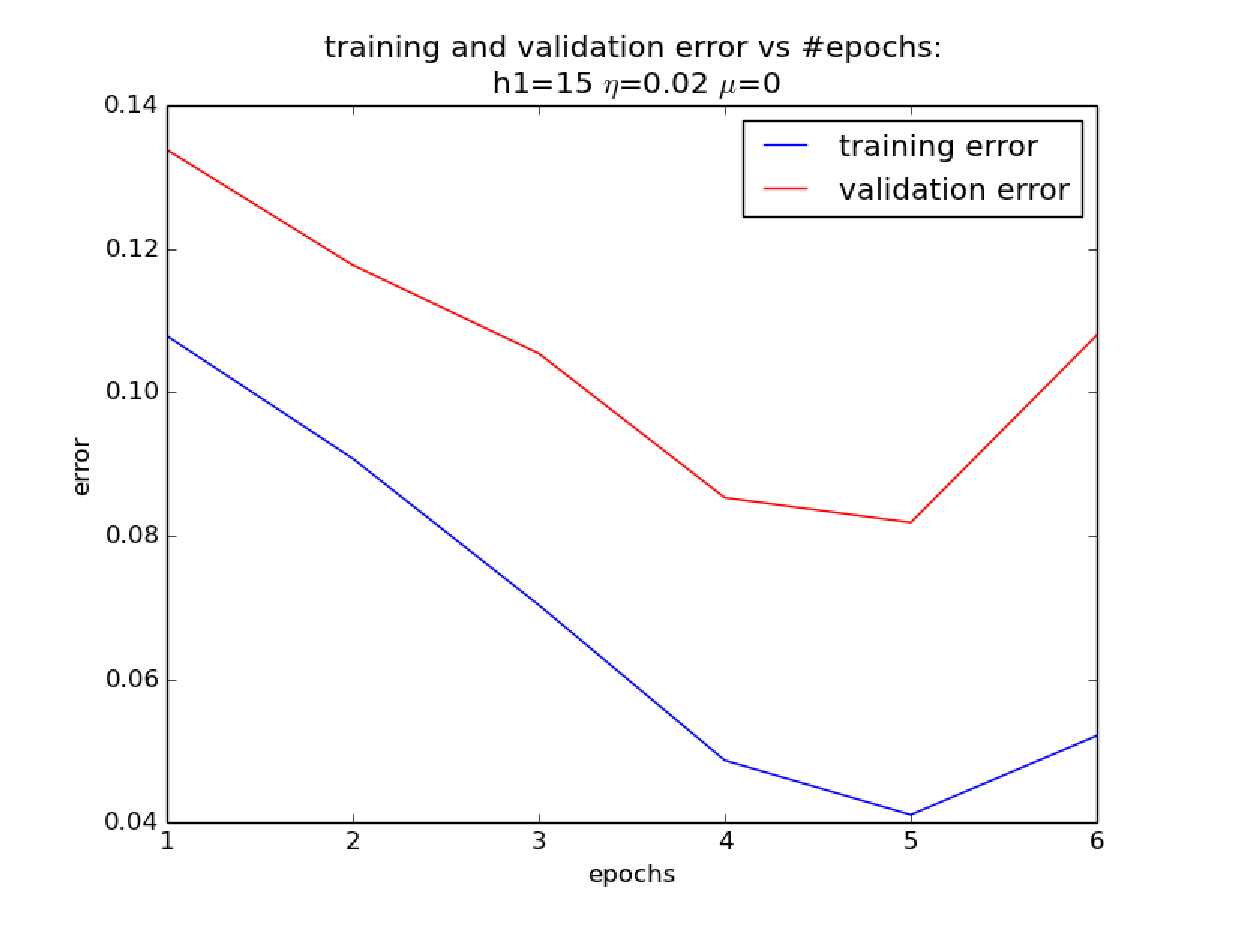
\includegraphics[width=\textwidth]{mlp/plots/effect_eta_larger.eps}
		\caption{Errors decrease with larger $\eta_0=0.02$}
		\label{fig:larger_eta}
		\end{subfigure}
		\begin{subfigure}[b]{.45\textwidth}
		\centering
		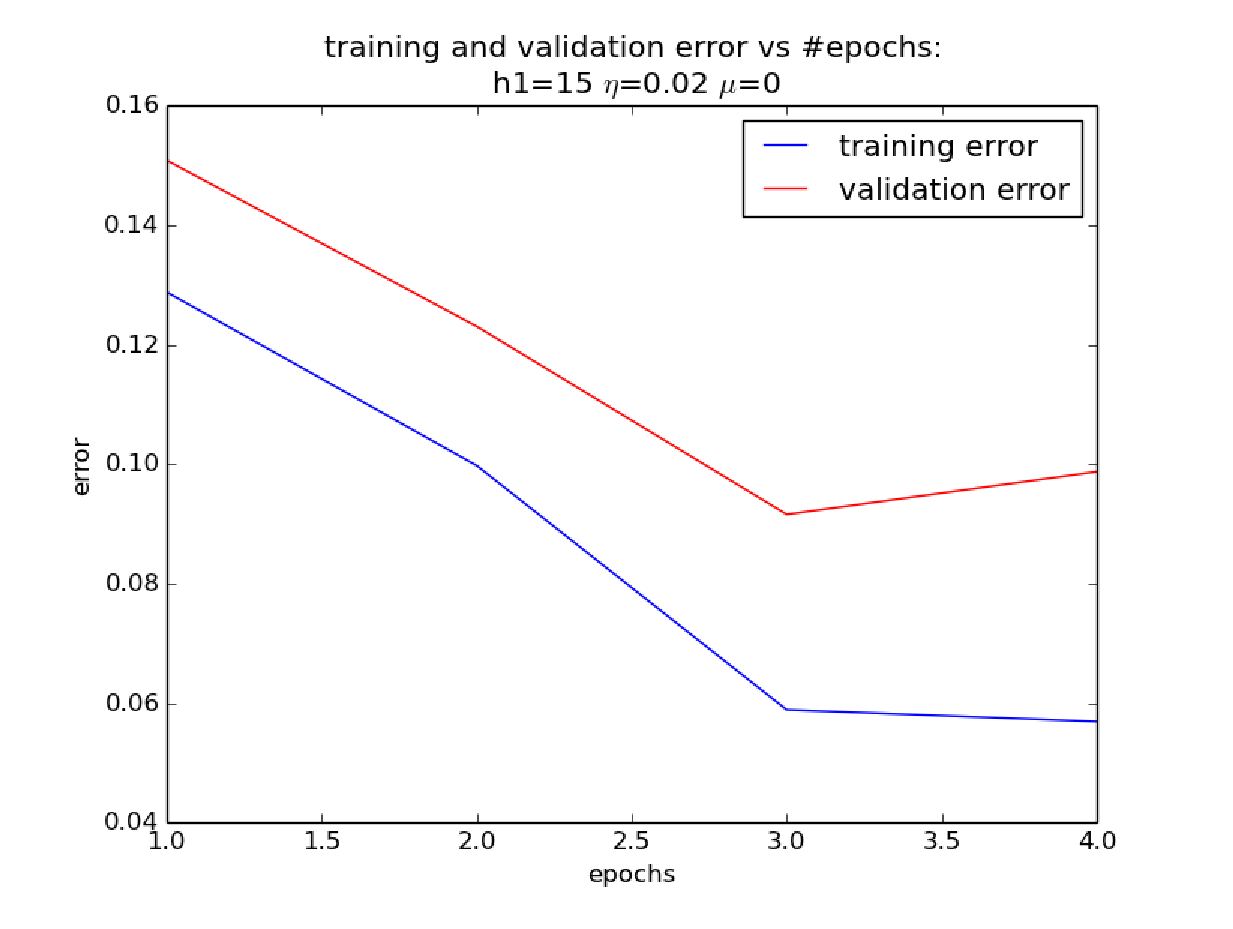
\includegraphics[width=\textwidth]{mlp/plots/effect_eta_decrease.eps}
		\caption{Decreasing $\eta$ after every epoch}
		\label{fig:decrease_eta}
		\end{subfigure}
		\quad
		\begin{subfigure}[b]{.45\textwidth}
		\centering
		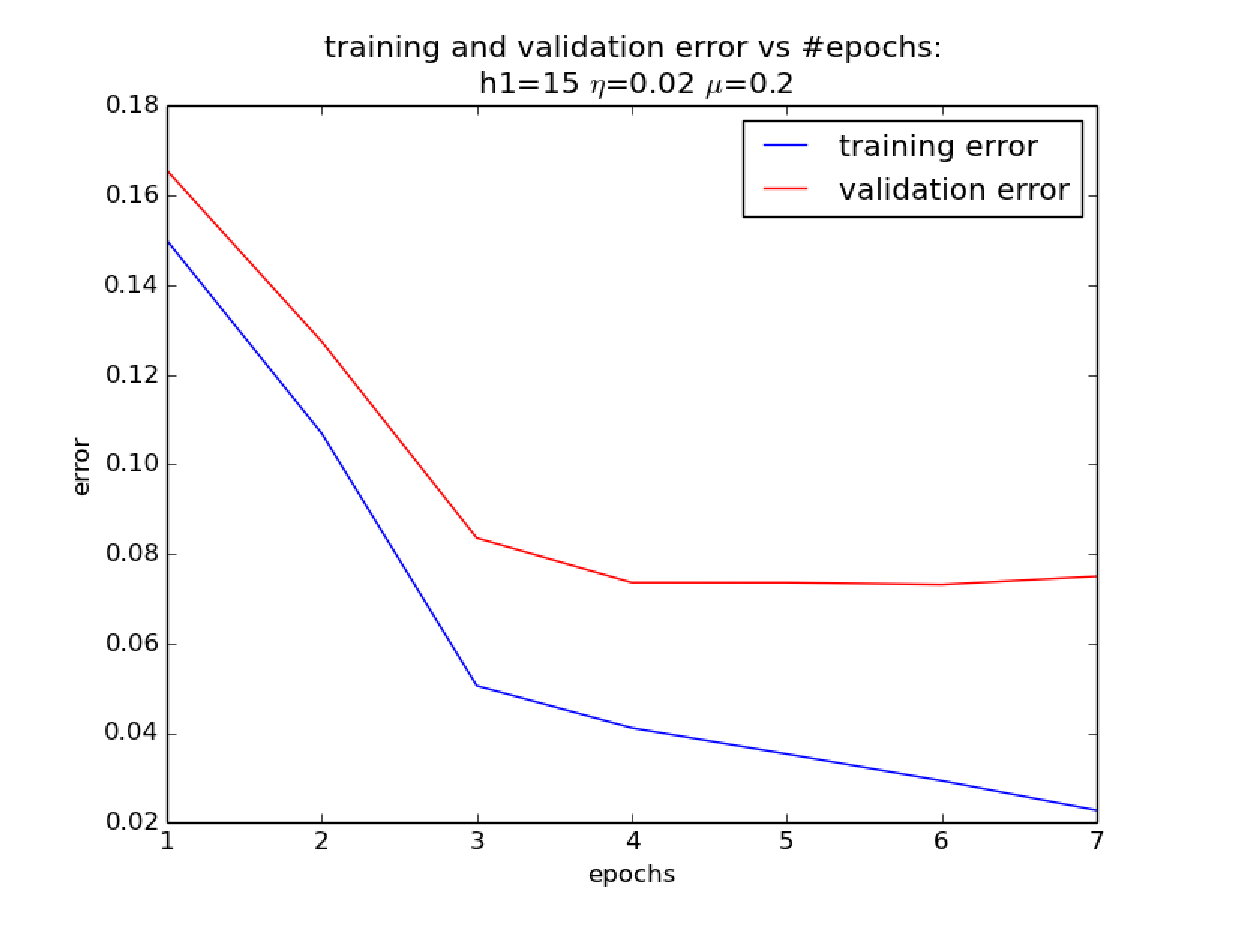
\includegraphics[width=\textwidth]{mlp/plots/effect_momentum.eps}
		\caption{Errors after introducing momentum term}
		\label{fig:increase_momentum}
		\end{subfigure}
		\caption{This figure exemplifies the effects of increasing the initial learning rate $\eta_0$ and then decreasing it every epoch, as well as the effect of introducing a momentum term stabilizing the gradient descent.}
		\label{fig:effects_learning_rate}
		\end{figure}
	By increasing the initial learning rate $\eta_0$ we were able to decrease the number of epochs, until an increase in the validation error occurs, to 6. After decreasing the learning rate in every epoch, the optimization converged already in the 4-th epoch. Introducing a momentum term $\mu = 0.2$ as in fig. \ref{fig:increase_momentum} result in a faster decrease of error values.

	\item Effects of number hidden units $h_1$
		\begin{figure}[!ht]
		\centering
		\begin{subfigure}[b]{.45\textwidth}
		\centering
		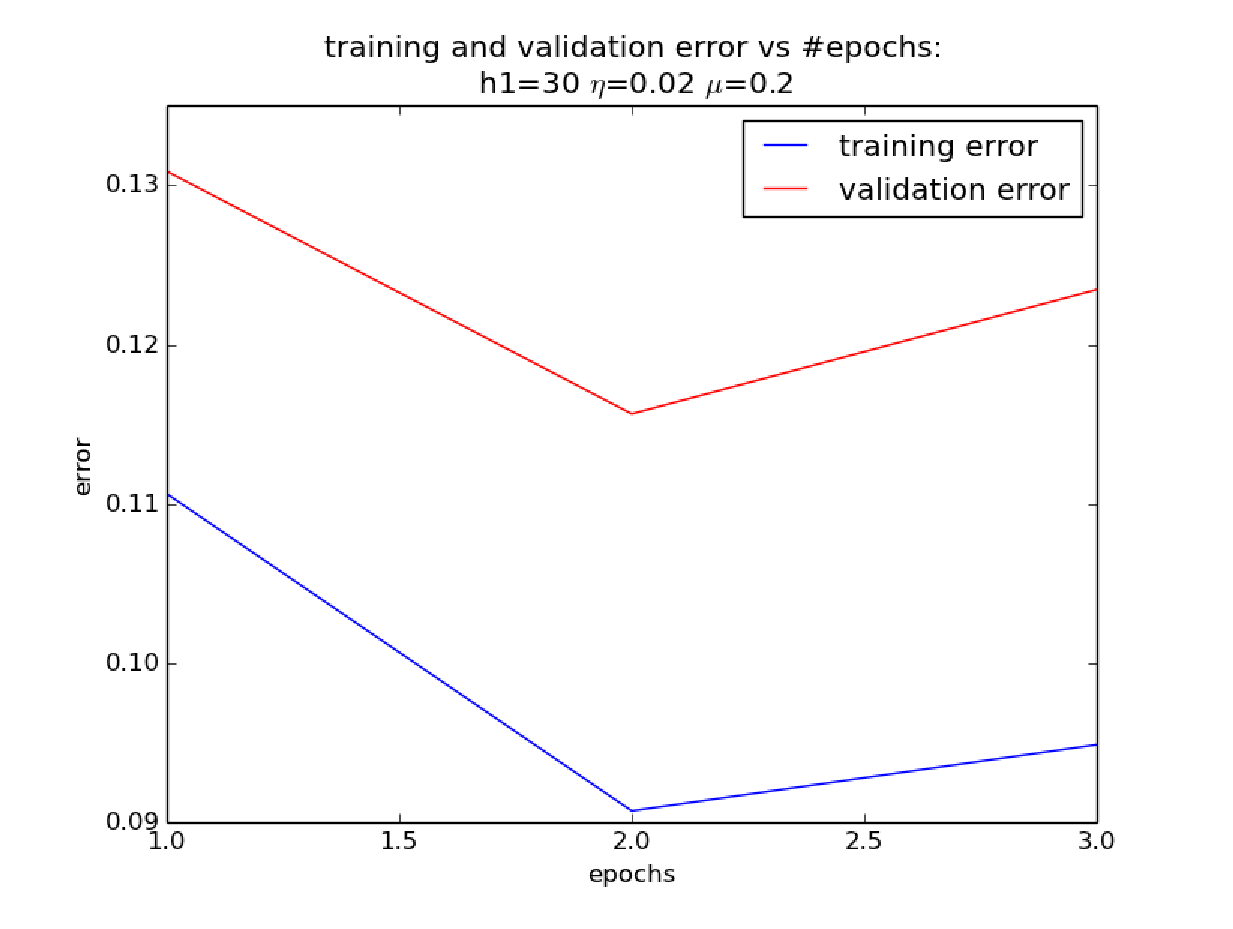
\includegraphics[width=\textwidth]{mlp/plots/30h1.eps}
		\caption{example subcaption}
		\end{subfigure}
		\quad
		\begin{subfigure}[b]{.45\textwidth}
		\centering
		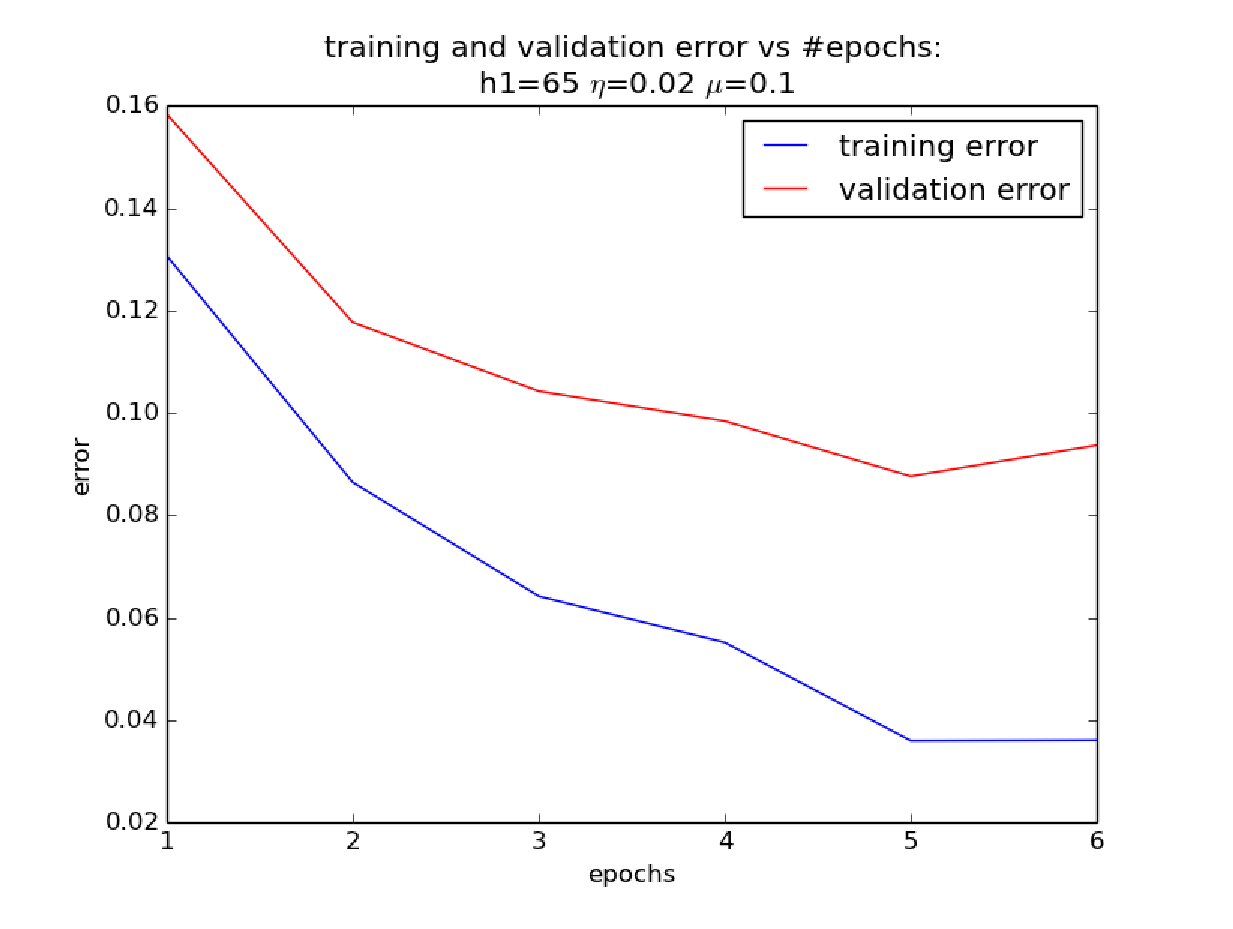
\includegraphics[width=\textwidth]{mlp/plots/65h1.eps}
		\caption{example subcaption}
		\label{fig:subfigure2}
		\end{subfigure}
		\quad
		\begin{subfigure}[b]{.45\textwidth}
		\centering
		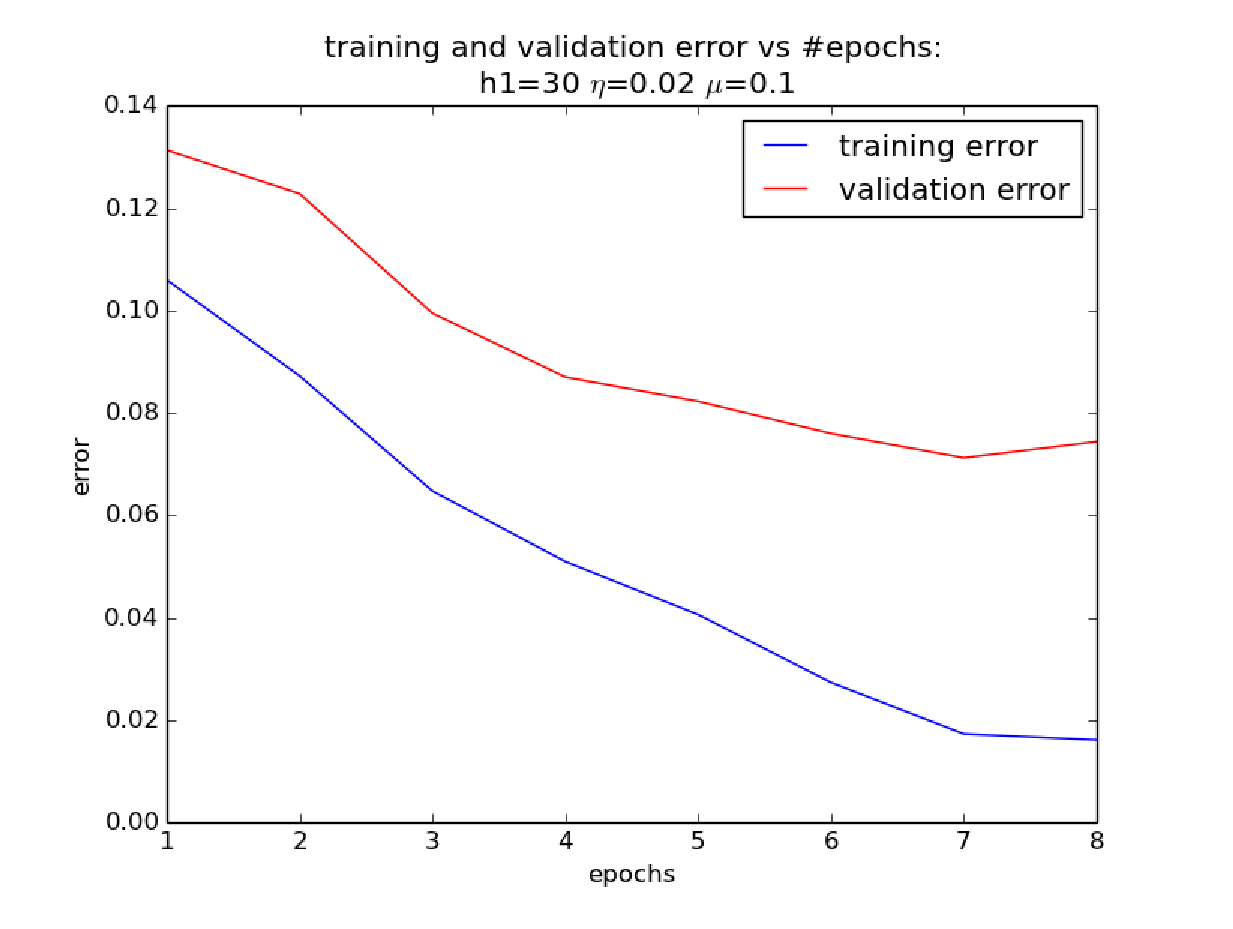
\includegraphics[width=\textwidth]{mlp/plots/30h1_tuned.eps}
		\caption{example subcaption}
		\label{fig:subfigure1}
		\end{subfigure}
		\quad
		\begin{subfigure}[b]{.45\textwidth}
		\centering
		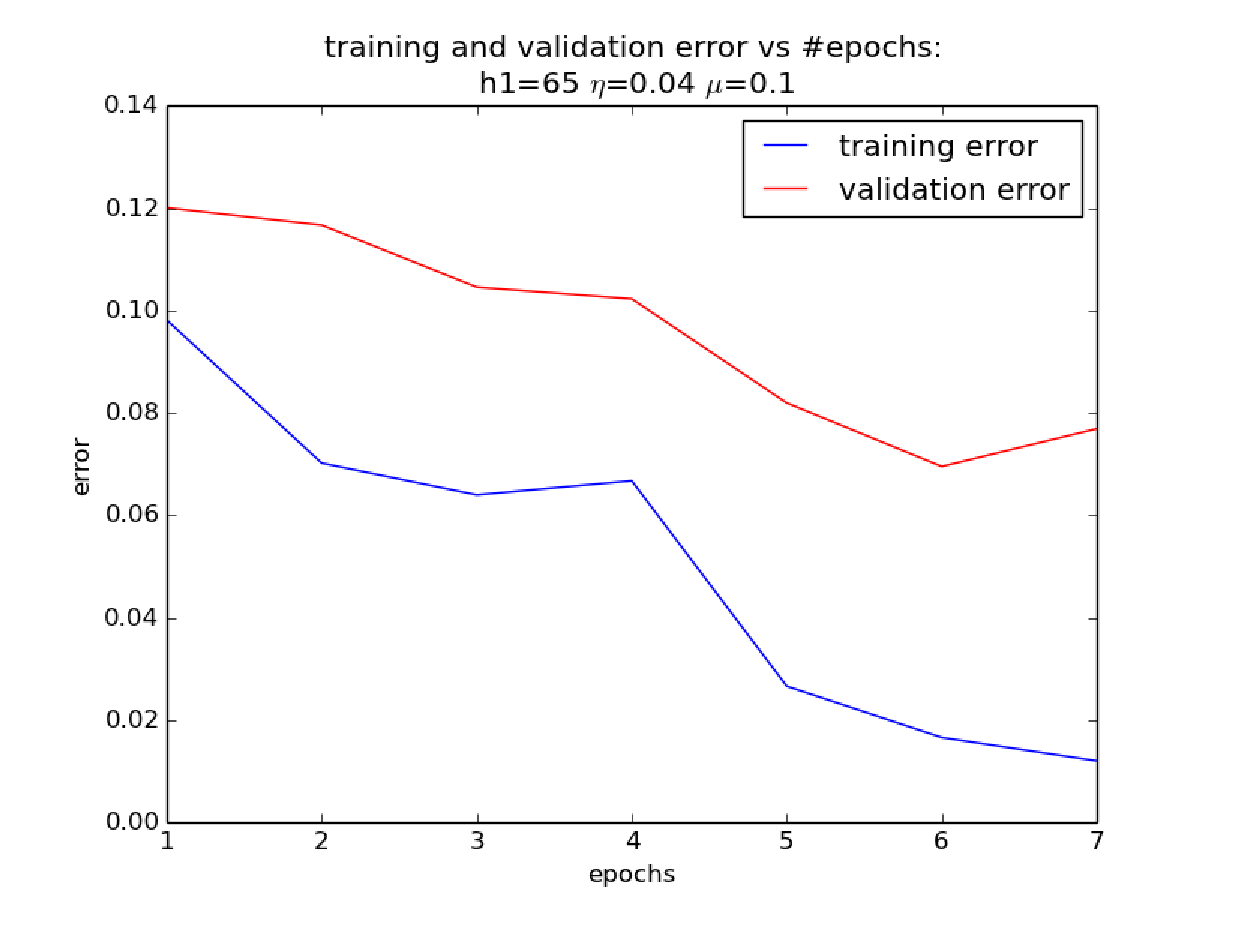
\includegraphics[width=\textwidth]{mlp/plots/65h1_tuned.eps}
		\caption{example subcaption}
		\label{fig:subfigure3}
		\end{subfigure}	
		\caption{Example caption}
		\label{fig:example}
		\end{figure}

\end{itemize}

\subsubsection{Effects of parameter choice on overfitting}
show for which parameters training error decreases while validation increases
yes, some epochs, not many... and you do this only for the report. in the learning algo, you would stop immediately
okwe actually got better results when running once over 98%
what do you mean?
over 98 is good!
with early-stopping we nearly never get more than 97.75%
so if you run 1 extra epoch after early stopping, it is better?
yes, like two or threebecause it increases and goes down again
that's a good finding!
write it in your report!
because there is no real danger of overfitting, because we use only 15 hidden inputsright?
very good!
in my case we used 64 units and we were overfitting if we would leave it for longer. We go more than 98 also
with small dimentionality it generalizes more. It's not the same, but you can look at it learning in higher dimentionality and throwing away the least significant dimentions(which usually overfit)
but it's not the same
	\begin{figure}[!ht]
	\centering
	\begin{subfigure}[b]{.45\textwidth}
	\centering
	\includegraphics[width=\textwidth]{mlp/placeholder.png}
	\caption{example subcaption}
	\end{subfigure}
	\quad
	\begin{subfigure}[b]{.45\textwidth}
	\centering
	\includegraphics[width=\textwidth]{mlp/placeholder.png}
	\caption{example subcaption}
	\end{subfigure}
	\caption{Example caption}
	\label{fig:overfiting}
	\end{figure}

include \textsc{typical} example of overfitting by letting the validation error increase while the training error decreases for a few, say 3, rounds!

\subsubsection{Determining parameters for binary subtasks}

\begin{figure}[!ht]
	\centering
	\begin{subfigure}[b]{.45\textwidth}
	\centering
	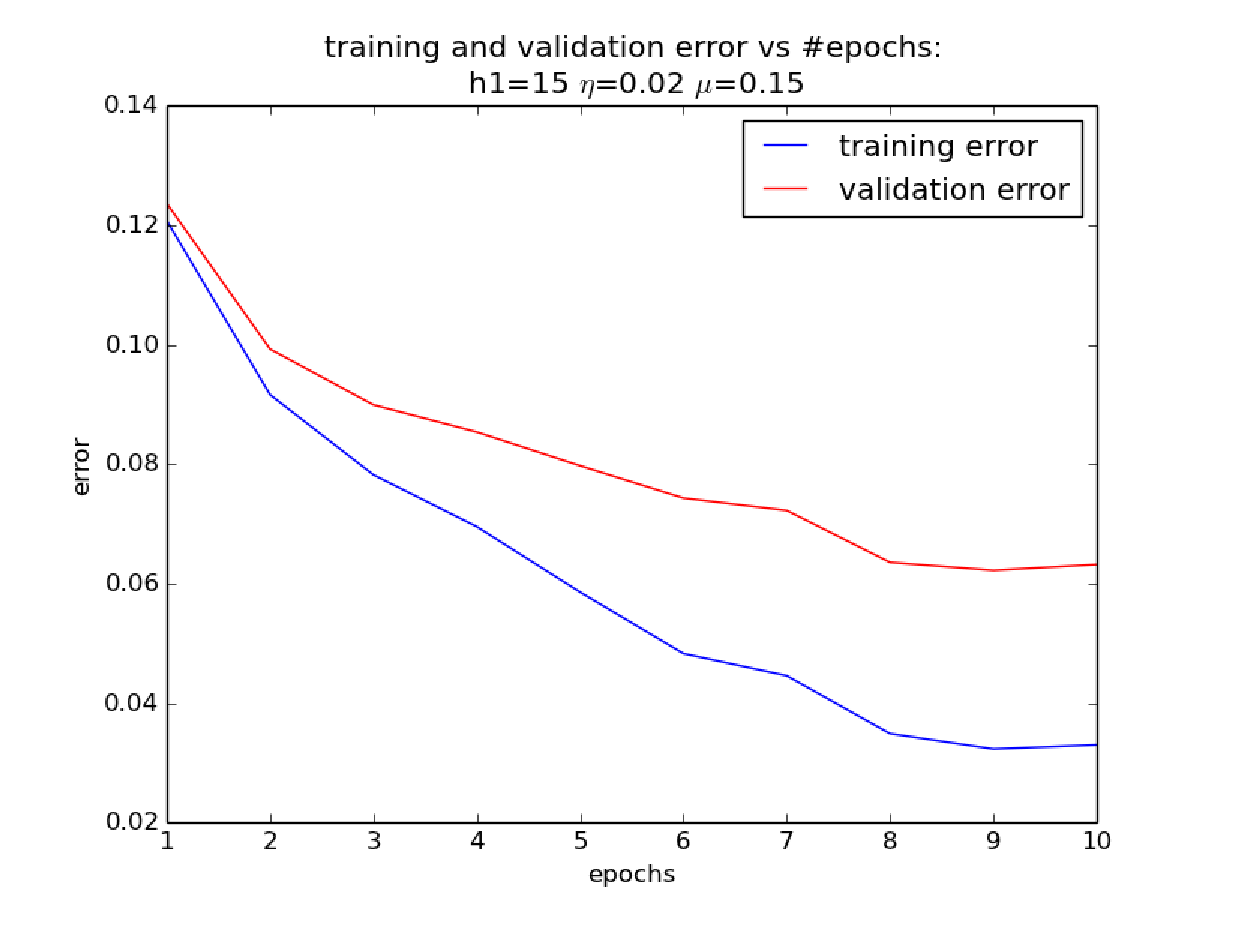
\includegraphics[width=\textwidth]{mlp/plots/4-9_tuned_97_75.eps}
	\caption{example subcaption}
	\label{fig:4_9_tuned}
	\end{subfigure}
	\quad
	\begin{subfigure}[b]{.45\textwidth}
	\centering
	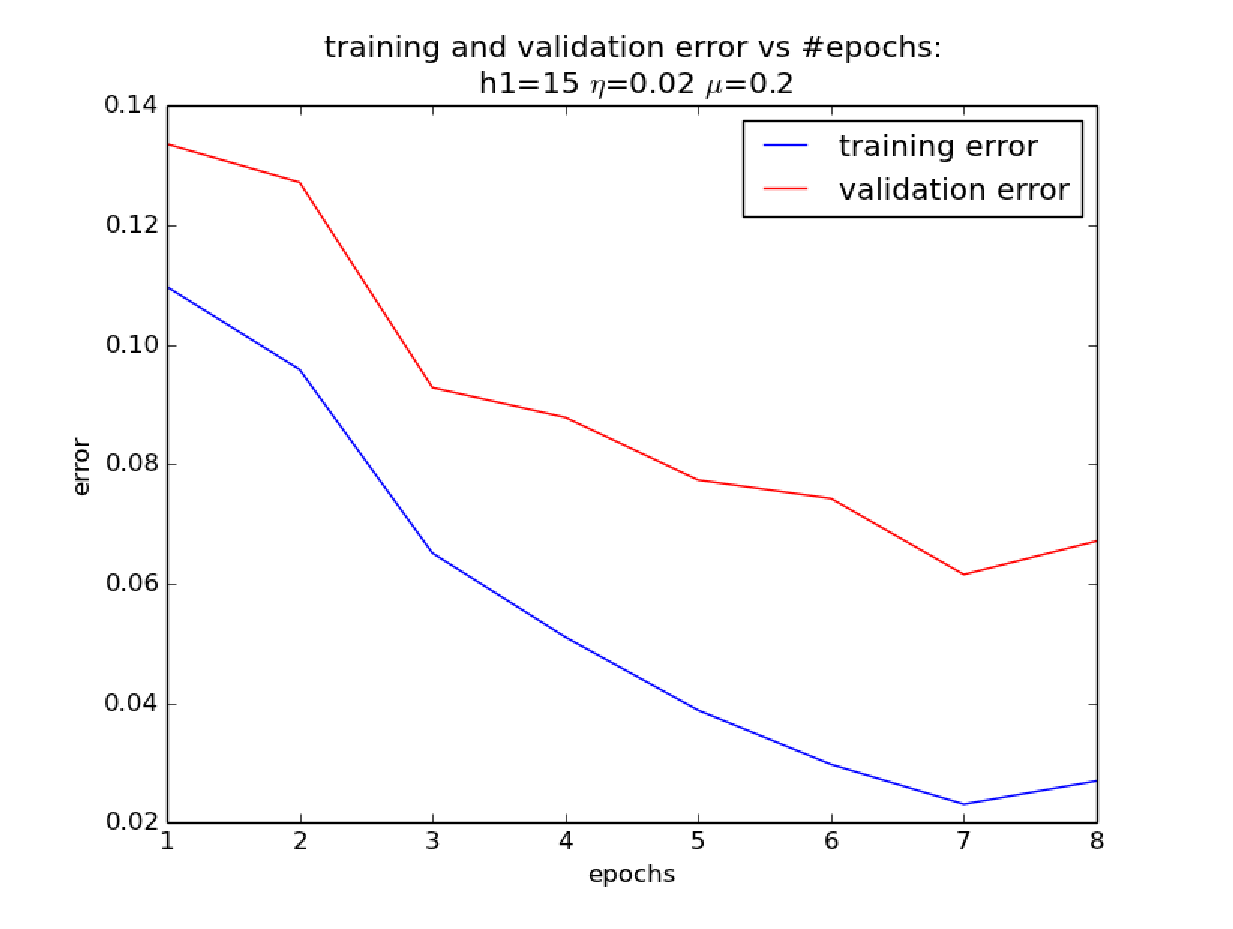
\includegraphics[width=\textwidth]{mlp/plots/3-5_tuned_97_75.eps}
	\caption{example subcaption}
	\label{fig:3_5_tuned}
	\end{subfigure}
	\quad
	\begin{subfigure}[b]{.45\textwidth}
	\centering
	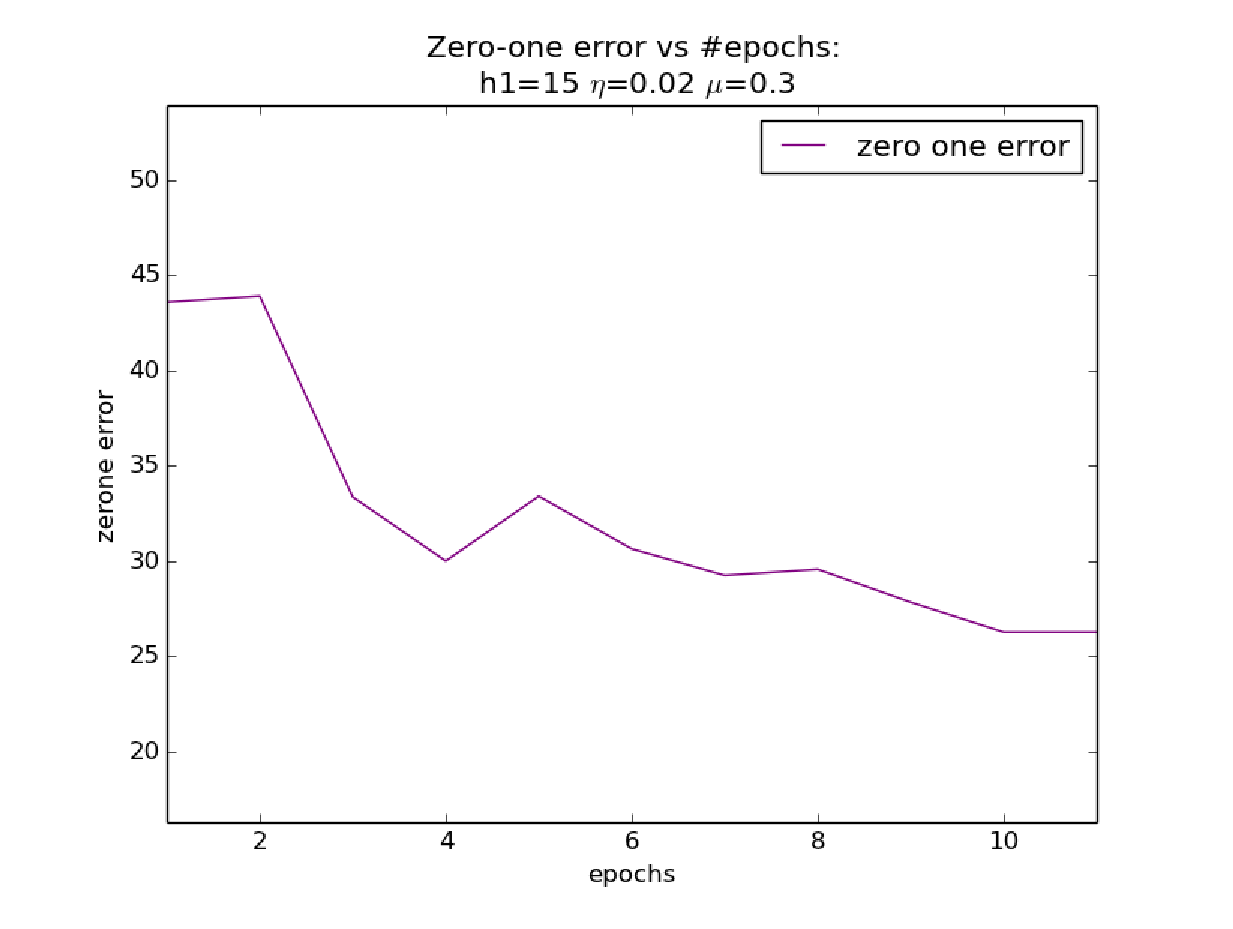
\includegraphics[width=\textwidth]{mlp/plots/zerone_optimize_4_9.eps}
	\caption{example subcaption}
	\label{fig:4_9_tuned_zerone}
	\end{subfigure}
	\quad
	\begin{subfigure}[b]{.45\textwidth}
	\centering
	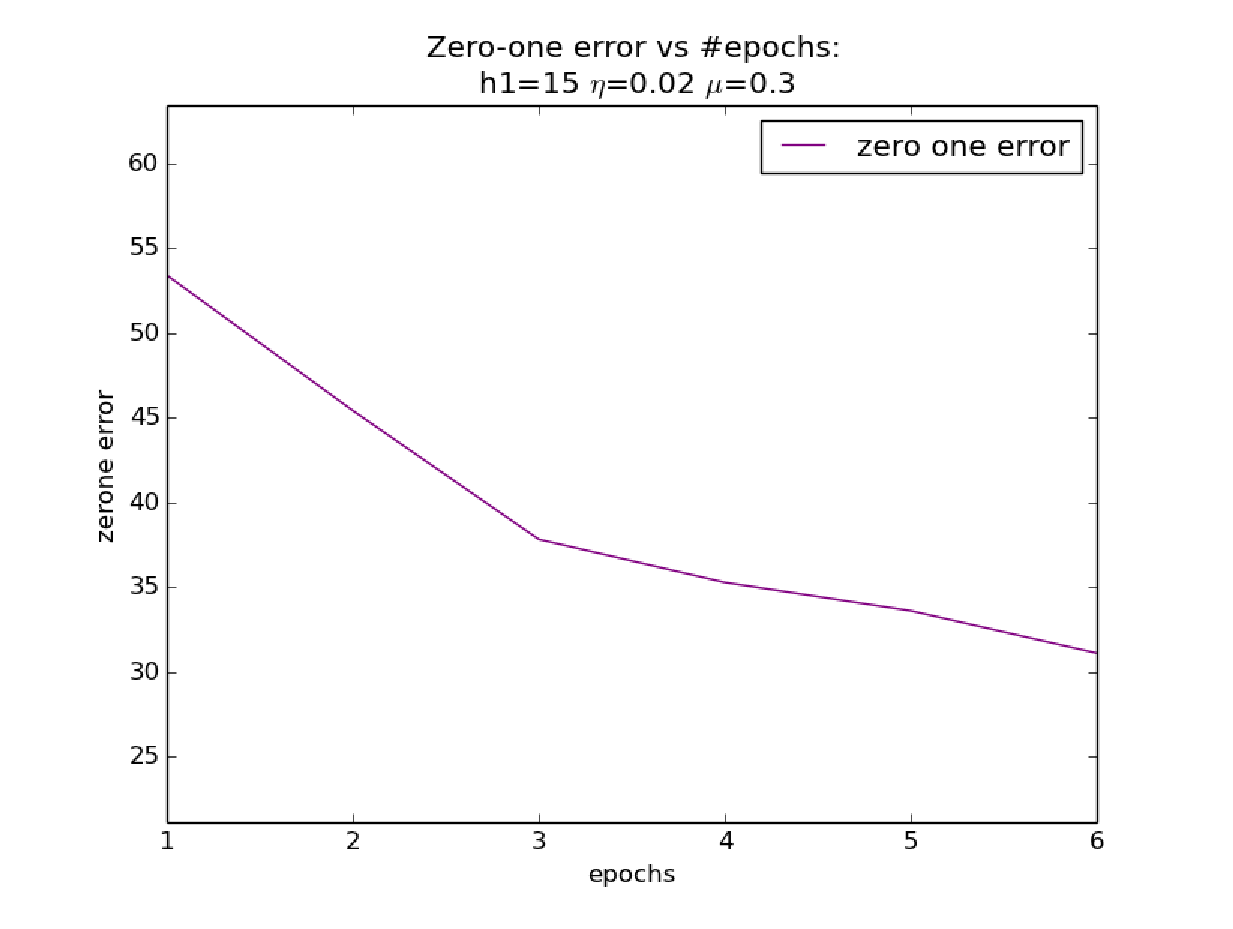
\includegraphics[width=\textwidth]{mlp/plots/zerone_optimize_3_5.eps}
	\caption{example subcaption}
	\label{fig:3_5_tuned_zerone}
	\end{subfigure}

	\caption{zerone}
	\label{fig:binary_subtasks}
\end{figure}
\textsc{Comment on findings \textbf{qualitatively}}		

\section{Results}
	plots annotated by the result of the final classifier on the test set
	\subsection{Discussion of performance on test set}

	\subsection{Misclassified patterns}
	\ref{fig:misclass_3} shows a misclassified point where ti*a2 is close to 0.
The actual label is -1, meaning that the data point represents a 9. The fact that is was misclassified by little  means that the model finds enough similarities with a 4. \ref{fig:misclass_4} shows a misclassified point where ti*a2 is far from 0.
The actual label is -1, the data point if for a 9. yet, the fact that a2 was greater than zero means the classifier sees it as a clear 4.
The point is actually an outlier from the "4 class" to the "9 class".
	\begin{figure}[!ht]
	\centering
	\begin{subfigure}[b]{.45\textwidth}
	\centering
	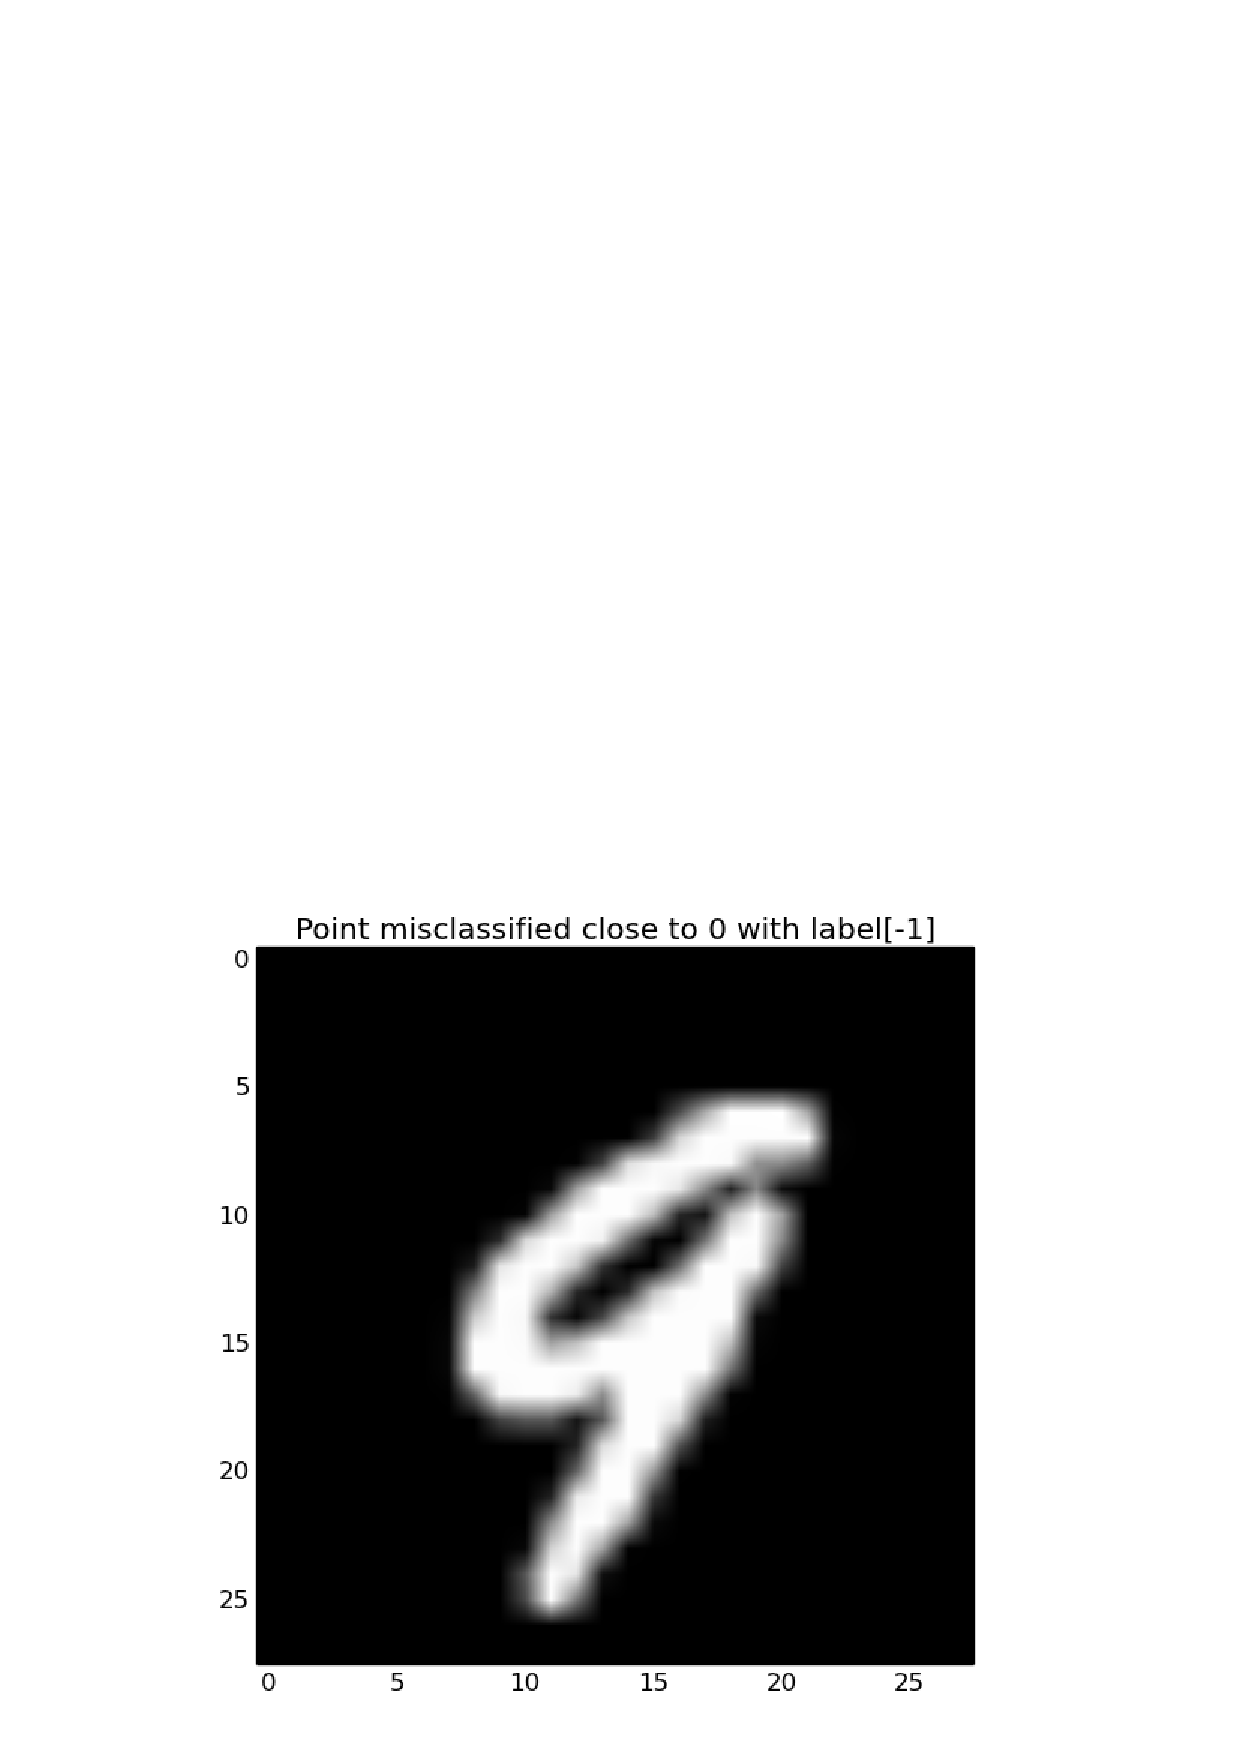
\includegraphics[width=\textwidth]{mlp/plots/misclassified_fig3.png}
	\label{fig:misclass_3}
	\caption{9 just about misclassified as a 4}
	\end{subfigure}
	\quad
	\begin{subfigure}[b]{.45\textwidth}
	\centering
	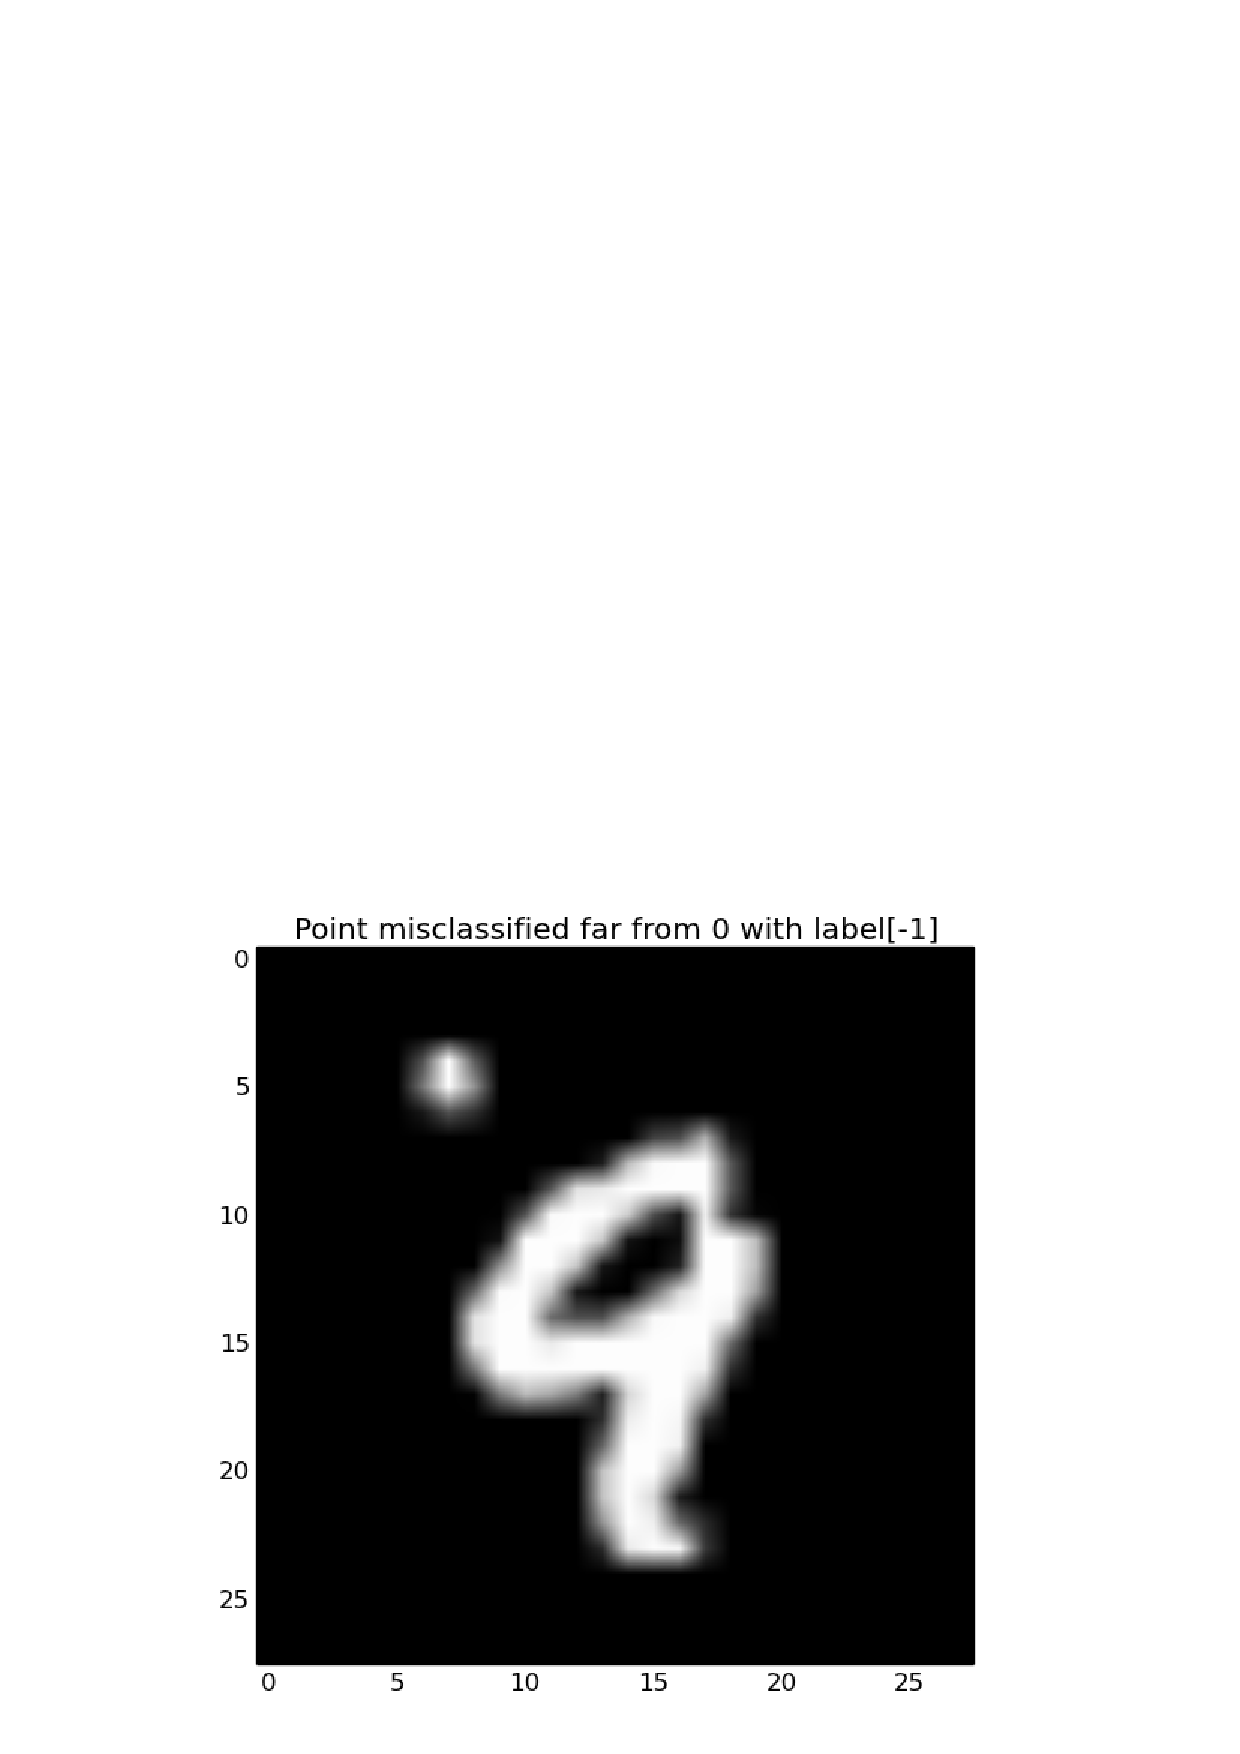
\includegraphics[width=\textwidth]{mlp/plots/misclassified_fig4.png}
	\label{fig:misclass_4}
	\caption{9 clearly mistaken as a 4 by classifier}
	\end{subfigure}
	\caption{Examples of misclassified patterns for 4-9 problem}
	\label{fig:misclassification}
	\end{figure}

